\documentclass{article}
\usepackage[utf8]{inputenc}
\usepackage[backend=biber,style=ieee,citestyle=numeric-comp]{biblatex} %for bibliography
\usepackage{array} % for table m
\usepackage{multirow} % tables
\usepackage{hyperref} % urls
\usepackage{underscore} % annoying -> seq ids
\usepackage{xspace} % spacing (copyright)
\usepackage{chngpage} % margin changes (species table)
\usepackage[list=true]{subcaption} % confusion matrix tables
\usepackage[title,titletoc]{appendix} % for appendices
\usepackage{chngcntr} % for section labels on tables and figures
% \usepackage{listings} % code and output listings
\usepackage{xcolor} % colors (for listings)
\usepackage[framemethod=tikz]{mdframed} % listings
\usepackage{capt-of} % for captions outside floats: listings
\usepackage{tocloft} % for defining custom lists (\listof)
\usepackage[ruled,vlined]{algorithm2e} % algorithms


% \lstset{  
% % language=Java,  
% % tabsize=4,  
% % basicstyle=\ttfamily,  
% % basicstyle=\linespread{1.1}\ttfamily\footnotesize,xleftmargin=0.7cm,
%     % frame=tlbr, framesep=0.2cm, framerule=0pt,
% % backgroundcolor=\color{lightgray},  
% % showstringspaces=false  
% }


% ccs concepts: feature selection, 

\addbibresource{references.bib}
\hypersetup{ colorlinks=true, urlcolor=black, linkcolor=black, citecolor=black } % urls

\patchcmd{\appendices}{\quad}{: }{}{} % appendix titles with colons
% WORK AROUND FOR INDENTED FOOTNOTE 
\makeatletter
\renewcommand\@makefntext[1]{%
\setlength\parindent{1em}%
\noindent
\mbox{\@thefnmark.~}{#1}}
\makeatother
% COMBINED LIST OF TABLES AND FIGURES (and listings and algorithms, etc)
% (requires capt-of and tocloft)
\newcounter{combinedfigure}
\newcounter{combinedtable}
\newcounter{combinedlisting}
\newcounter{combinedalgorithm}

\makeatletter
\@addtoreset{combinedtable}{section}
\@addtoreset{combinedlisting}{section}
\@addtoreset{combinedfigure}{section}
\@addtoreset{combinedalgorithm}{section}
\makeatother

\newcommand{\stepcombinedcounter}[1]{
\ifstrequal{#1}{Table}{\refstepcounter{combinedtable}}{}
\ifstrequal{#1}{Listing}{\refstepcounter{combinedlisting}}{}
\ifstrequal{#1}{Figure}{\refstepcounter{combinedfigure}}{}
\ifstrequal{#1}{Algorithm}{\refstepcounter{combinedalgorithm}}{}
}

\newcommand{\combinedcounter}[1]{%
\ifstrequal{#1}{Table}{\thecombinedtable}{}%
\ifstrequal{#1}{Listing}{\thecombinedlisting}{}%
\ifstrequal{#1}{Figure}{\thecombinedfigure}{}%
\ifstrequal{#1}{Algorithm}{\thecombinedalgorithm}{}%
}

\newcommand{\combinedlistname}{\Large List of Tables and Figures}
\newlistof{combined}{combined2}{\combinedlistname}

\newcommand{\figcaption}[2]{%
\par\stepcombinedcounter{#1}%
\captionof*{table}{#1~\thesection.\combinedcounter{#1}: #2}%
\addcontentsline{combined2}{combined}{\textbf{#1~\thesection.\combinedcounter{#1}} #2}%
}

% when TOC should exclude some text from caption
\newcommand{\figcaptionalt}[3]{%
\par\stepcombinedcounter{#1}%
\captionof*{table}{#1~\thesection.\combinedcounter{#1}: #2}%
\addcontentsline{combined2}{combined}{\textbf{#1~\thesection.\combinedcounter{#1}} #3}%
}
% for bib: make citeauthor link
\DeclareCiteCommand{\citeauthor}
  {\boolfalse{citetracker}%
   \boolfalse{pagetracker}%
   \usebibmacro{prenote}}
  {\ifciteindex
     {\indexnames{labelname}}
     {}%
   \printtext[bibhyperref]{\printnames{labelname}}}
  {\multicitedelim}
  {\usebibmacro{postnote}}
  
\DeclareCiteCommand{\citeyear}
  {\boolfalse{citetracker}%
   \boolfalse{pagetracker}%
   \usebibmacro{prenote}}
  {\ifciteindex
     {\indexnames{labelname}}
     {}%
   \printtext[bibhyperref]{\printfield{year}}}
  {\multicitedelim}
  {\usebibmacro{postnote}}
 
\newcommand{\textcitecomma}[1]{(\citeauthor{#1}, \citeyear{#1})}
\renewcommand{\textcite}[1]{\citeauthor{#1} (\citeyear{#1})}

\title{The Role of Machine Learning in SARS-CoV-2 Susceptibility Classification}
\author{Zak White}
\date{April 22, 2022}

% code marathon
\begin{document}
\pagenumbering{roman}
\vspace*{8em}
\newcommand\tpbreak{\\[\baselineskip]}
\thispagestyle{empty}

\begin{center}
    THE ROLE OF MACHINE LEARNING IN\\ SARS-CoV-2 SUSCEPTIBILITY CLASSIFICATION
 \tpbreak
    by \tpbreak
    Zak White \\
    University of Victoria \tpbreak
    A graduating thesis submitted in partial fulfilment of the requirements for the Honours degree of \tpbreak
    BACHELOR OF SCIENCE \tpbreak
    in the Department of Computer Science
    
    \vfill
    
    \textcopyright\xspace 2022 Zak White \\
    University of Victoria \tpbreak    
    All rights reserved. This thesis may not be reproduced in whole or in part, by photocopying or other means, without the permission of the author. \tpbreak
    We acknowledge with respect the Lekwungen peoples on whose traditional territory the university stands and the Songhees, Esquimalt, and WSANEC peoples whose historical relationships with the land continue to this day.
\end{center}


\newpage

\vspace*{8em}
\begin{center}
    THE ROLE OF MACHINE LEARNING IN\\ SARS-CoV-2 SUSCEPTIBILITY CLASSIFICATION \tpbreak
    by \tpbreak
    Zak White \\
    University of Victoria
\end{center}

% \vfill

\section*{Abstract}
\addcontentsline{toc}{section}{Abstract}

SARS-CoV-2 is a contagious virus established to affect not only humans, but other mammal species. Studies over the last two years have revealed certain species are distinctly immune to the virus, which can be attributed to differences in the ACE2 protein, the virus' target protein, in various hosts. This study applies machine learning methods to classify hosts as susceptible or immune to SARS-CoV-2 based on their ACE2 sequences.

\vspace{1em}\noindent
Machine learning has faced criticism within the field of biology for its uninterpretable logic; it's imperative that biologists and medical professionals can have confidence in the tools they use, and this isn't always possible with machine learning. This is an investigation into the importance of explainable machine learning within bioinformatics that involves the comparison of three models with varying degrees of biological considerations.

\vspace{1em}\noindent
This study validated the hypothesis that biology-driven machine learning applications outperform pure machine learning models, and produced other interesting findings on how mutations in the ACE2 protein can affect susceptibility to SARS-CoV-2.


\newpage
\tableofcontents
\addcontentsline{toc}{section}{Table of Contents}

\newpage
\listofcombined
\addcontentsline{toc}{section}{List of Tables and Figures}

\newpage
\section*{Acknowledgments}
\addcontentsline{toc}{section}{Acknowledgments}

I would like to thank:

My thesis supervisor \textbf{Dr. Hosna Jabbari} for offering me the opportunity to perform this research, inspiring the project topic, and for her guidance through the process. Further, the members of the \textbf{Computational Biology Research and Analytics (COBRA)} group at the University of Victoria for their resources and feedback.

\textbf{My supportive friends.}

Most profoundly, \textbf{my parents and family} for their endless unconditional support and love at every step of my life leading to this academic achievement.

% Thank you to Dr. Hosna Jabbari (for inspiration, guidance, introduction to concepts, and COBRA)

% Thank you to Tibor and/or Tracey.

% Thank you to my loving friends.

% Thank you to my parents.

\newpage
\section*{Dedication}
\addcontentsline{toc}{section}{Dedication}
\emph{To Isla.}

\vspace{1em}

\noindent\emph{Everything in this world is yours.}

\newpage
\
\newpage
\pagenumbering{arabic}
\newpage\section{Introduction}

For over two years, the COVID-19 pandemic has been a headline research topic as it inescapably invades our world and affects our lives in unparalleled ways. COVID-19 is a disease caused by severe acute respiratory
syndrome coronavirus 2 (SARS-CoV-2), a virus believed have
zoonotic origins \cite{Andersen2020}.

Since its discovery, SARS-CoV-2 studies have identified a range of animal hosts --- including some nonhuman primates,  mustelids, bats, and felines --- that can be infected by and can transmit the virus \cite{Luan2020,Woolsey2020,OIE2022,OudeMunnink2021,Schlottau2020,Sreenivasan2020,Leroy2020}. Conversely, certain research has supported the conclusion that other species (e.g. the domestic pig) are explicitly immune to the virus \cite{Luan2020,Sreenivasan2020,Zhao2020,Shi2020}. This disjunction promotes the question: \emph{what makes some species susceptible to the virus and others immune?} Investigating this question has been an ongoing focus in bioinformatics to mitigate interspecies transmission.

The answer might correspond to how the the virus interacts with its target protein in different hosts. The SARS-COV-2 spike protein’s target is the angiotensin-converting enzyme 2 (ACE2). Differences in the ACE2 sequence can affect the spike protein’s binding affinity, thus affecting the host’s susceptibility to the virus.

\begin{figure}[h]
    \centering
    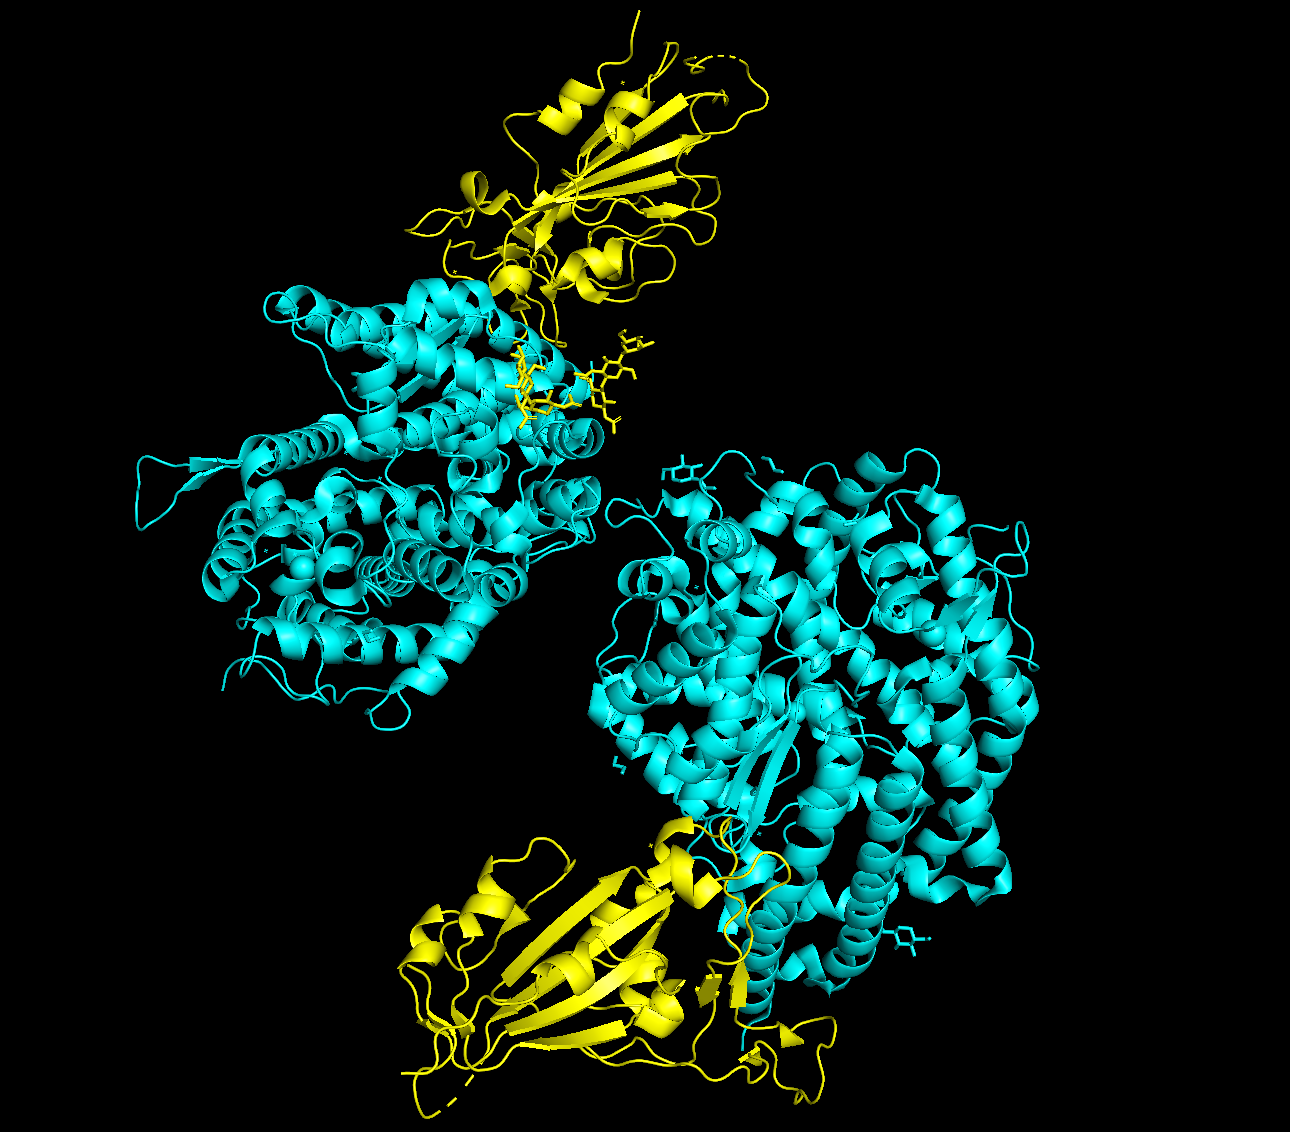
\includegraphics[width=0.8\textwidth]{figures/RBD-interaction.png}
    \figcaptionalt{Figure}{Structure of SARS-CoV-2 spike protein (yellow) complexed with its target ACE2 (cyan)}{SARS-CoV-2 spike protein complexed with its target ACE2}
\end{figure}

\subsection{Machine Learning}

Machine learning is a branch of artificial intelligence used to build models for classification or decision-making based on data, without explicit programming. Nowadays, machine learning is used across industrial fields to plan, make correct decisions, and increase the efficiency of the processes \cite{Mottaqi2021}. 

Within the field of biology, machine learning has outperformed human analysis in certain tasks. For example, in 2018, \citeauthor{Kakadiaris2018} designed a support-vector machine model for classifying risk of cardiovascular disease that produced an accuracy of over 85\% and missed fewer disease events than the US guidelines' manual risk calculator.

Despite its success, the use of machine learning within biology has been met with criticism. Models, especially black-box models (where the internal working is not revealed), have been condemned for their uninterpretable logic, and for not being paired with a biological explanation \cite{Rudin2019}. Bioinformatic problems often represent high-stakes decisions (e.g. diagnoses), so it is imperative that models used to address the problems can be trusted from a biological standpoint.

\subsection{Sequence Classification}

Proteins are biomolecules that comprise chains of organic compound units known as amino acids. There are twenty amino acids, each of which can be represented using a letter character. By defining a protein as a sequence of characters corresponding to the amino acid chain, the sequence can be used as a feature vector for classification. Take the human ACE2 sequence, built of a chain of 805 acid residues:

\[ MSSSSW...DVQTSF \]

\noindent where each letter corresponds to a distinct acid (methionine as $M$, serine as $S$, etc.). The sequence can be converted into a feature vector:

\[ x = (M,S,S,S,W,...,D,V,Q,T,S,F) \]

\noindent which can be used for classification. The features are categorical (limited to a fixed set of values) and nonordinal (there is no logical sorting order). 

The basis of this study is using the amino acid feature vectors of a protein to classify sequences as susceptible or immune to SARS-CoV-2.

\subsection{Objective and Contribution}

This study is an investigation into the validity of machine learning for classifying sequence susceptibility to SARS-CoV-2, to gain insight into the validity of machine learning as a bioinformatic tool at a higher level.

Three classification models are designed:
\begin{itemize}
    \setlength\itemsep{0em}
    \item a \textbf{baseline} machine learning model;
    \item an \textbf{eliminative} machine learning model; and
    \item a \textbf{structural} model that incorporates the findings of a protein structure analysis
\end{itemize}

The models are tested against a set of host protein sequences to evaluate their performances. It is hypothesized that the structural model will outperform its machine learning counterparts as the more accurate classifier.

\subsection{Related Work}

Machine learning has been growing in popularity for sequence classification \cite{Iqbal2014}, but an ongoing barrier is the magnitude of the feature vectors: proteins can be built of hundreds or thousands of amino acids, so reducing the problem to a manageable number of features can be challenging \cite{Saidi2010}. Bioinformaticians including \textcite{Iqbal2014} and \textcite{Saidi2010} have developed methods for feature selection specifically designed for reducing size of the feature vector of protein sequences, each leading to models that outperform standard machine learning tools.   

\textcite{Patel2016} reported linear discriminant analysis was a more accurate method than support vector machines, naive Bayes, and logistic regression when classifying amino acid sequences as secretory or not. Discriminant analysis involves applying statistical methods to find a set of features that best separates the classes \cite{Abdi2007}. The principals of discriminant analysis were implemented in the machine learning models of this study: training sequences were analyzed to identify which acids were most influential to susceptibility, and those acids were used as indicators for susceptibility in the models. 

Many studies have included structural investigations into how changes in the ACE2 sequence affects binding with the SARS-CoV-2 spike protein:
\begin{itemize}
    \setlength\itemsep{0em}
    \item In an overview of ACE2 and its function, \textcite{Li2021} reported major interaction sites including positions 24-42, 79-83, and 353-357, emphasizing positions 38, 41, 42, 82, 83, 353, and 355.
    \item \textcite{Zhao2020} investigated the effect of mutations in 23 critical sites, highlighting the effects of positions 24, 27, 30, 31, 34, 41, 79, 82, 83, 325, 329, and 353.
    \item \textcite{Luan2020} consolidated the results of existing structural analyses and used their findings to predict the host range of the virus (the set of species the virus is capable of infecting), focusing on the acids in positions 31, 35, 38, 82, and 353.
\end{itemize}

\newpage\section{Method}

\subsection{Data}
Fourty-one ACE2 sequences from various animal hosts were collected from the NCBI protein database\footnote{\url{https://www.ncbi.nlm.nih.gov/protein}}. Each host has been identified as either susceptible or insusceptible to the virus, based on:
\begin{itemize}
    \setlength\itemsep{0em}
    \item investigations into non-human primates as models for human
    infection;
    \item research into potential origin species (bats, pangolins);
    \item lab studies that assessed binding affinities between the SARS-CoV-2 spike protein and ACE2 in various hosts;
    \item studies focusing on transmission between humans and livestock, house pets, and city animals; and
    \item reports on city and zoo animals contracting the virus.
\end{itemize}

Additional sequences were collected to classify hosts whose susceptibilities are unknown. Each sequence was aligned with the human ACE2 sequence using the Needleman-Wunsch algorithm (via the EMBOSS Needle pairwise sequence alignment tool\footnote{\url{https://www.ebi.ac.uk/Tools/psa/emboss_needle/}}) to produce an optimal global alignment. This preprocessing step ensured that indexing of each sequence correlated to that of the human ortholog.

For the structural analysis, three protein models were retrieved from the AlphaFold Protein Structure Database\footnote{\url{https://alphafold.ebi.ac.uk/}}, and one structure modelling the interaction between the SARS-CoV-2 spike protein and human ACE2 was retrieved from the RCSB Protein Data Bank\footnote{\url{https://www.rcsb.org/}}.

Exhaustive lists of sequences are attached in Appendix A.

\subsection{Baseline Model}

First, a baseline classification model was created using a feature importance algorithm which scored the acids at each index as a feature. This step was implemented using the scikit-learn\footnote{\url{https://scikit-learn.org/}} machine learning package's univariate feature selection tools, with the features scored using chi-squared tests with a 97.5\% confidence threshold ($\alpha = 0.025$). 

This algorithm identified which acids in the training data had the greatest effect on susceptibility, and the results were used to create a categorical binary decision tree.

\subsection{Eliminative Model}

A second model was designed by extending on the results of an existing study \textcitecomma{White21} that focused on mutations that eliminate binding affinity between ACE2 and the SARS-CoV-2 spike protein. The original analysis involved an iterative algorithm that isolated mutations that appeared exclusively in immune sequences (Algorithm 2.1).

\begin{algorithm}[ht]
  \NoCaptionOfAlgo
  \SetAlgoLined
  \For {each immune sequence $S^-$}{
    \For {each i \textless length of $S^-$} {
        $isInfluentialIndex \leftarrow$ True\;
        \For {each susceptible sequence $S^+$}{
            \If {$i^{th}$ acid in $S^-$ == $i^{th}$ acid in $S^+$}{
            $isInfluentialIndex \leftarrow$ False\;
            }
        }
        \If {isInfluentialIndex} {
            \tcp{The mutation may be influential}
            Record $i$, $i^{th}$ acid in $S^-$
        }
    }
  }
  \figcaption{Algorithm}{Finding potential influential mutations} 
%   \vspace{-32pt}
\end{algorithm}


The mutations were scored based on frequency in immune sequences and inversely based on the total number of mutations in the sequence. The mutations with scores that exceeded a defined threshold ($\alpha = 0.5$) were used as the basis for another binary decision tree.

\subsection{Structural Model}

A reduced model was created by pairing the findings of the eliminative model with a structural analysis, with the goal of removing extraneous results. For each mutation identified in the original work used for the previous model, a manual structural investigation into the mutation was conducted using the molecular visualization tool PyMOL\footnote{\url{https://pymol.org/}}, involving:

\begin{itemize}
    \setlength\itemsep{0em}
    \item comparing the structure of the mutated sequence with the structure of the human ACE2 sequence.
    % \item investigating how the mutation affects the surrounding structure (neighbouring acids). 
    \item looking at a model of the spike protein binding with human ACE2 to understand if the position may be a binding site.
\end{itemize}

\subsection{Model Comparison}

The classification models were evaluated using testing sets of different lengths: the baseline model was tested against seven sequences (80/20 train/test split), the eliminative model was tested against 26 sequences (the subset of sequences that were not used in the original study), and the structural model was tested using the full set of 41 sequences.

The testing sets were used to produce confusion metrics for each model, from which performance sensitivity, specificity, and accuracy were derived. These performance metrics were used to compare the models.

Two types of pairwise statistical hypothesis tests were performed to determine if there was statistical difference between models:
\begin{itemize}
    \setlength\itemsep{0em}
    \item Two-sample tests for equality of proportions were used for sensitivity and specificity.
    \item McNemar's tests were used for error rate.
\end{itemize}

\newpage\section{Results}

%     maybe misclassifications of each model and show each index and highlight where the model focuses.
%     31/41/82/.../679 m1 m2 m3 actual
%     A  F  P /.../ G  +  -  +  +
%     negative emphasized there.
\subsection{Preliminary Results}

The feature selection algorithm for the baseline model found six sites that best discriminate the susceptibility of the training sequences (Table 3.1). Each position has specific set of amino acids that increase likelihood of a sequence being immune.

\begin{table}[ht]
  \centering
  \begin{tabular}[t]{ c | l }
    \hline
    \textbf{Pos} & \textbf{Acids that impede susceptibility} \\
    \hline
    83 & Phenylalanine (F) \\
    211 & Aspartate (D) \\
    212 & Alanine (A), Aspartate (D), Serine (S) \\
    246 & Arginine (R) \\
    251 & Valine (V) \\
    687 & Not Alanine (A) or Serine (S) \\
    \hline
  \end{tabular}
  \figcaption{Table}{Summary of feature selection algorithm results}
\end{table}

The eliminative algorithm based on the original study identified eight mutations that only appeared in immune sequences, shown in Table 3.2.

\begin{table}[ht]
  \centering
  \begin{tabular}[t]{ c | c  c  c }
    \hline
    \textbf{Pos} & \multicolumn{3}{c}{\textbf{Mutation}} \\
    \hline
    31 & Lysine (K) & $\to$ & Aspartate (D){\rule{0pt}{2.6ex}} \\[1mm]
    41 & Tyrosine (Y) & $\to$ & Alanine (A) \\[1mm]
    \multirow{2}{*}{66} & Glycine (G) & \multirow{2}{*}{$\Rightarrow$} & \multirow{2}{*}{Alanine (A)} \\
    & Arginine (R) \\[1mm]
    83 & Tyrosine (Y) & $\to$ & Phenylalanine (F) \\[1mm]
    \multirow{2}{*}{113} & Serine (S) & \multirow{2}{*}{$\Rightarrow$} & \multirow{2}{*}{Asparagine (N)} \\
    & Arginine (R) \\[1mm]
    353 & Lysine (K) & $\to$ & Histidine (H) \\[1mm]
    426 & Proline (P) & $\to$ & Serine (S) \\[1mm]
    679 & Isoleucine (I) & $\to$ & Valine (V) \\[1mm]
    \hline
  \end{tabular}
  \figcaption{Table}{Mutations that may abolish susceptibility (eliminative)}
\end{table}

\subsection{Structural Analysis}

By complementing the findings of the preliminary findings with a structural analysis, the feature set used for the structural model was reduced to five sites. 

\begin{figure}[ht!]
    \centering
    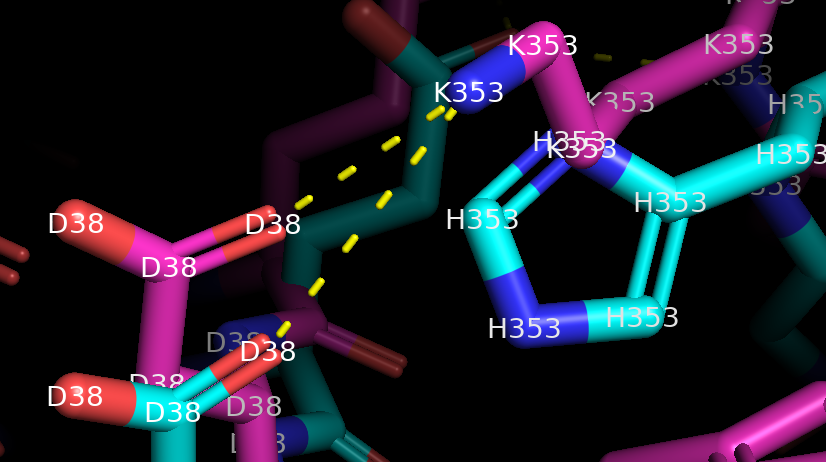
\includegraphics[width=\textwidth]{figures/structure-353.png}
    \figcaption{Figure}{The structural effect of mutation H353}
\end{figure}

As an sample of the findings of the investigation, Figure 3.1 depicts the change caused by the mutation at position 353 from lysine (K) to histidine (H). The human ortholog is coloured pink, and the rat ortholog containing the mutation is coloured cyan. This mutation abolishes a polar bond between the residue at position 353 and the aspartate (D) at position 38. Further, the lysine at position 353 in the human sequence displayed potential to bond with the virus spike protein, suggesting it may be a binding site. Since the mutation had an affect on the structure of the protein and there is evidence it may be a binding site, the mutation was included in the structural model. 

\begin{table}[ht]
  \centering
  \begin{tabular}[t]{ c | c  c  c }
    \hline
    \textbf{Pos} & \multicolumn{3}{c}{\textbf{Mutation}} \\
    \hline
    31 & Lysine (K) & $\to$ & Aspartate (D){\rule{0pt}{2.6ex}} \\[1mm]
    83 & Tyrosine (Y) & $\to$ & Phenylalanine (F) \\[1mm]
    \multirow{2}{*}{113} & Serine (S) & \multirow{2}{*}{$\Rightarrow$} & \multirow{2}{*}{Asparagine (N)} \\
    & Arginine (R) \\[1mm]
    353 & Lysine (K) & $\to$ & Histidine (H) \\[1mm]
    426 & Proline (P) & $\to$ & Serine (S) \\[1mm]
    \hline
  \end{tabular}
  \figcaption{Table}{Mutations that may abolish susceptibility (structural)}
\end{table}

The list of mutations used for the structural model is depicted in Table 3.3, and a more detailed overview of the structural analysis involved is included in Appendix B.

\subsection{Model Design}

With the set of mutations that abolish susceptibility identified for each model, three categorical binary decision trees were made for classification. Table 3.4 outlines the subset of positions selected for use in each model.

\begin{table}[ht]
  \centering
  \begin{tabular}[t]{ c | c  c  c | c }
    \hline
    & \multicolumn{3}{c|}{Model} \\
    \textbf{Pos} & \textbf{B} & \textbf{E} & \textbf{S} & \textbf{UniProt} \\
    \hline
    31 & & \texttimes & \texttimes & \texttimes \\
    41 & & \texttimes & & \texttimes \\
    66 & & \texttimes & & \\
    83 & \texttimes & \texttimes & \texttimes & \texttimes \\
    113 & & \texttimes & \texttimes & \\ 
    211 & \texttimes & & & \\
    212 & \texttimes & & & \\ 
    246 & \texttimes & & & \\
    251 & \texttimes & & & \\
    353 & & \texttimes & \texttimes & \texttimes \\
    426 & & \texttimes & \texttimes & \texttimes\\
    679 & & \texttimes & & \\
    687 & \texttimes & & & \\
    \hline
  \end{tabular}
  \figcaption{Table}{Positions of focus for each model}
\end{table}

Each marked cell indicates the position was used as a feature in the model of the column, where B, E, and S represent the baseline, eliminative, and structural models, respectively. The UniProt column is marked for each position where the UniProt database's mutagenesis overview identified the position as influential to susceptibility \cite{UniProt}. The UniProt database consolidates the findings of many studies to summarize how mutations affect susceptibility; this column represents a standard of comparison for the feature set of each model.

It is clear from this table that the structural model was most true to the findings outlined on UniProt, while the baseline model was not similar at all.

\subsection{Model Performance}

Each model was evaluated using its corresponding test set to produce confusion matrices (Table 3.5). The rows of the matrices represent the true class of the sequences, and the columns represent the model's predicted class.

\begin{table}[!htb]
    \figcaption{Table}{Classification confusion matrices for each model}
    \begin{subtable}{.33\linewidth}
      \centering
        \begin{tabular}{c|c|c}
            & + & -  \\
            \hline
            + & 5 & 1 \\
            - & 1 & 1 \\
        \end{tabular}
      \caption{Baseline Model}
    \end{subtable}%
    \begin{subtable}{.33\linewidth}
      \centering
        \begin{tabular}{c|c|c}
            & + & -  \\
            \hline
            + & 14 & 3 \\
            - & 3 & 6 \\
        \end{tabular}
      \caption{Eliminative Model}
    \end{subtable}%
        \begin{subtable}{.33\linewidth}
      \centering
        \begin{tabular}{c|c|c}
            & + & -  \\
            \hline
            + & 24 & 3 \\
            - & 5 & 9 \\
        \end{tabular}
      \caption{Structural Model}
    \end{subtable}%
\end{table}

The sensitivity (true positive rate), specificity (true negative rate), and accuracy for each model were computed based on the confusion matrices (Table 3.6). The structural model had the highest accuracy and sensitivity, meaning it was more successful than the other models at correctly identifying sequences that are susceptible, and more successful at classifying sequences overall \cite{Vu2015}. The eliminative model had a marginally higher specificity.

\begin{table}[ht]
  \centering
  \begin{tabular}[t]{ c | c  c  c }
    \hline
    \textbf{Model} & \textbf{Sensitivity} & \textbf{Specificity} & \textbf{Accuracy} \\
    \hline
    Baseline & 0.83 & 0.50 & 0.75 \\
    Eliminative & 0.82 & 0.67 & 0.77 \\
    Structural & 0.89 & 0.64 & 0.80 \\
    \hline
  \end{tabular}
  \figcaption{Table}{Accuracy metrics for each model}
\end{table}

Pairwise two-sample tests for equality of proportions used to compare sensitivities and specificities revealed no statistically significant difference between the performances of the models. Further, McNemar's tests used to compare error rates found no statistical difference between the misclassification rates of models \cite{Vu2015, PatrickWalters2021, Crawley2015}.

Formulae and equations used for computing performance metrics are included in Appendix C, and a summary of statistical tests is included in Appendix D.  
% look into https://en.wikipedia.org/wiki/Total_operating_characteristic
\newpage\section{Discussion}

Revisiting the positions selected as features for each model (Table 3.4), the structural model was almost completely in agreement with the UniProt findings --- the exceptions were positions 41 and 113. Position 41 was excluded from the model arbitrarily: among the data used for this study, no sequences featured mutations at position 41. Position 113 was included in the eliminative model, and kept in the structural model because of the change in structure caused by the mutation to asaparagine (N). This disconnect between the positions in the model and the UniProt findings could mean this is a novel mutation that affects susceptibility, or it could be an extraneous finding attributed to an imperfect structural analysis.

The structural model's positions of focus were most similar to the UniProt findings, but the eliminative model also shared a considerable overlap: five of eight positions in the feature set appeared on the UniProt overview, and four appeared in this study's related work \cite{Li2021,Zhao2020,Luan2020}. This is surprising, especially given the limited size of training data provided for the eliminative algorithm, and suggests the algorithm has some validity.

A well-trained and -tested model could be used to predict susceptibility in hosts where it is not already known. Table 4.1 shows the classifications of new sequences for each model.

\newcommand{\prediction}[5]{#1 (\emph{#2}) & #3 & #4 & #5 }

\begin{table}[h!]
    \centering
    \begin{tabular}{lccc}
        \hline
        \textbf{Species} & \textbf{B} & \textbf{E} & \textbf{S} \\
        \hline
        \prediction{Chinchilla}{chinchilla lanigera}{\texttimes}{}{} \\
        \prediction{Grizzly bear}{ursus arctos horribilis}{\texttimes}{\texttimes}{\texttimes} \\
        \prediction{Black flying fox}{pteropus alecto}{}{\texttimes}{\texttimes} \\
        \prediction{Sumatran orangutan}{pongo abelii}{\texttimes}{\texttimes}{\texttimes} \\
        \prediction{Tasmanian devil}{sarcophilus harrisii}{}{}{} \\
        \prediction{Orca}{orcinus orca}{\texttimes}{\texttimes}{\texttimes} \\
        \prediction{Turkey}{meleagris gallopavo}{}{}{} \\
        \prediction{Leatherback sea turtle}{dermochelys coriacea}{}{}{} \\
        \hline
    \end{tabular}
    \figcaption{Table}{Predicted classification of additional sequences}
\end{table}

The eliminative and structural models made the same predictions for each sequence. Focusing on where the models classified differently, it can be argued the eliminative and structural models' classifications were more intuitive based on existing knowledge:
\begin{itemize}
    \setlength\itemsep{0em}
    \item based on other rodents being immune (mice, rats), it would make sense for the chinchilla to be;
    \item based on other bats being susceptible, it would make sense for the black flying fox to be.
\end{itemize}

The structural model outperformed the other models in terms of classification accuracy, but the eliminative model was a close second. This further validates the algorithm used to identify influential mutations for features in the eliminative model. 

Although the eliminative model did not involve any biological considerations, it performed similarly to the improved structural model which did; this suggests there is some rationality to the use of machine learning for this problem. The underachievement of the baseline model suggests the univariate feature selection strategy is not as suitable, at least given the training size.

\subsection{Limitations}

The greatest restriction of this study was the limited amount of data available surrounding species’ susceptibilities to the virus; SARS-CoV-2 is ever-topical and more information about spike protein and ACE2 interaction is still surfacing. The consequence of this limitation is a high risk of overfitting, less accurate models, and less confidence in performance metrics.
% mention that higher sample size improves chances of finding statistical difference
% "Your data should be randomly selected from a population, where each item has an equal chance of being selected." is an assumption for comparing proportions so the comparisons of spec/sens might not be perfect... lol. (sequence diversity can't be ensured)

Another limitation is the categorical and nonordinal nature of the features: the acids cannot be represented as numbers, nor can they be logically sorted. This severely restricts the variety of machine learning methods that can be used for the problem.

\subsection{Future Direction}

There are variations on the original problem that could be interesting for future work, specifically:

\begin{itemize}
    \item A \textbf{multinomial classification} model that categorizes sequences into degrees of susceptibility (i.e., immune, moderately susceptible, very susceptible). The UniProt mutagenesis summary for ACE2 highlights that some mutations abolish interaction with the spike protein, while others inhibit or increase interaction to various extents \cite{UniProt}. In the structural model, the hamster sequences was misclassified as immune by its serine at position 426, which has been identified as a mutation that only slightly inhibits interaction with the spike protein \cite{UniProt,Li2005}, not abolishing interaction as the model assumes. 
    \item A \textbf{multi-label classification} model that classifies hosts as susceptible, symptomatic, zoonotically potential (transmittable to humans), and/or intraspecies transmittable. Among the set of animals known to be susceptible to SARS-CoV-2, some have been identified as asymptomatic, and some unlikely to transmit the virus to humans or other hosts of the same species \cite{OIE2022,Singh2021}.
    \item A model with a \textbf{multidimensional feature space}. Each of the twenty amino acids can be categorized based on polarity, charge, and molecular size. Rather than focusing on the specific acid at each position, the model could classify the sequence based on these characteristics.
\end{itemize}
% Also, same as before with the mutations in multiple in a row having an effect. Like 82-84. If i looked at all of them structurally (include graphic here of 83 with bridge to 79 or whatever) then it could be more accurate. Also the effects 425-427 together have been specificalyl researched (we can see that the combined effects of 426 and 427 make for a structural differnce in the rat ortholog).
% Clustering
A more involved structural analysis could improve the performance of the structural model, specifically its specificity if more mutations that affected structure were identified. The analysis used for this model was based on the findings of the existing study used for the eliminative model, but extending beyond that set of mutations could reveal more potential influential positions. The analysis could be further strengthened by investigating the effect of mutations at consecutive positions; existing studies have reported consecutive mutations at sites 82-84 and 425-427 that each inhibit interaction with the spike protein \cite{Li2005,Li2021,UniProt}.
% -> look at more sites for structure differences
% -> compare with spike protein
% -> compare effect of consecutive mutations
\newpage\section{Conclusion}

When facing high-stakes decision --- a reality of biology --- having confidence in the tools that influence the decision is essential. When using black-box models, the logic is hidden and inherently less trustworthy; but even white-box models, where the logic is revealed, are not immediately trustworthy when not paired by an intuitive explanation.

The problem of using machine learning to classify sequences as susceptible or immune to SARS-CoV-2 is severely limited by the availability of data. Regardless, this analysis showed that it is possible to use existing data to classify sequences somewhat reliably: the eliminative model achieved an accuracy of 77\%, comparable to the maximum accuracy of 80\% of the structural model.

The hypothesis of this study was validated: the structural model marginally outperformed its counterparts. Equally significantly, this study is an example of how machine learning can be used as a starting point for classification models, and that pairing it with biological reasoning can strengthen their performances.


% blackbox bad, sometimes whitebox bad: just because you understand the logic of a model, doesn't mean you can understand why the model does that, and it's important to trust the process involved in high-stakes decision-making
% Hyptothesis met/validated, it's so important for biologists to be confident in the tools theyre working with, high stakes decisions,  This is not a great ML problem tho in general because of limited data, but this demonstrates some validity to the use of ML for sequence classification in general
\newpage\newpage
\section*{Data and Code Availability}
\addcontentsline{toc}{section}{Data and Code Availability}

The repository for this project is on GitHub (\url{https://github.com/zakwht/sars-cov-2}), within which is contained:

\begin{itemize}
    \setlength\itemsep{0em}
    \item the Python code used for all machine learning aspects of the project;
    \item the R code used for statistical analysis;
    \item some of the PyMOL script used for the structural analysis; and
    \item the processed data used for the project.
\end{itemize}

\noindent
The set of data used for this analysis is listed in Appendix A.

\newpage
\printbibliography
\addcontentsline{toc}{section}{References}

\newpage
\begin{appendices}

\section{Sequence Lists}
\newcommand{\spec}[5]{#1 (\emph{#2}) & \href{https://www.ncbi.nlm.nih.gov/protein/#3}{#3} & #4 #5 }

\newcommand{\cA}{\cite{Luan2020}}
\newcommand{\cB}{\cite{Zhao2020}}
\newcommand{\cC}{\cite{Leroy2020}}
\newcommand{\cD}{\cite{Richard2020}}
\newcommand{\cE}{\cite{OudeMunnink2021}}
\newcommand{\cF}{\cite{Palmer2021}}
\newcommand{\cG}{\cite{Chan2020}}
\newcommand{\cH}{\cite{OIE2022}}
\newcommand{\cI}{\cite{Sreenivasan2020}}
\newcommand{\cJ}{\cite{Shi2020}}
\newcommand{\cK}{\cite{Lu2020}}
\newcommand{\cL}{\cite{Woolsey2020}}
\newcommand{\cM}{\cite{Schlottau2020}}

\enlargethispage{2em}
\begin{table}[ht!]
    \begin{adjustwidth}{-12em}{-12em}
    \centering
    \begin{tabular}{lcc}
        \hline
        \textbf{Species} & \textbf{Accession} & \textbf{Susceptible} \\
        \hline
        \spec{Dromedary}{camelus dromedarius}{XP_031301717.1}{No}{\cA} \\
        \spec{Raccoon}{procyon lotor}{BAE72462.1}{No}{\cA} \\
        \spec{Greater horseshoe bat}{rhinolophus ferrumequinum}{XP_032963186.1}{No}{\cA} \\
        \spec{Brown rat}{rattus norvegicus}{NP_001012006.1}{No}{\cA\cB} \\
        \spec{House mouse}{mus musculus}{NP_001123985.1}{No}{\cA\cB} \\
        \spec{Platypus}{ornithorhynchus anatinus}{XP_001515597.2}{No}{\cA} \\
        \spec{African bush elephant}{loxodonta africana}{XP_023410960.1}{No}{\cA} \\
        \spec{European hedgehog}{erinaceus europaeus}{XP_007538670.1}{No}{\cA} \\
        \spec{Raccoon dog}{nyctereutes procyonoides}{ABW16956.1}{No}{\cA} \\
        \spec{Meerkat}{suricata suricatta}{XP_029786256.1}{No}{\cA} \\
        \spec{Kangaroo rat}{dipodomys ordii}{XP_012887573.1}{No}{\cA} \\
        \spec{Guinea pig}{cavia porcellus}{XP_023417808.1}{No}{\cA} \\
        \spec{Domestic pig}{sus domesticus}{ASK12083.1}{No}{\cI\cJ} \\
        \spec{Mallard}{anas platyrhynchos}{XP_012949915.3}{No}{\cI\cJ} \\
        \spec{Human}{homo sapiens}{BAB40370.1}{Yes}{} \\
        \spec{Rhesus macaque}{macaca mulatta}{XP_028697658.1}{Yes}{\cA\cB} \\
        \spec{European rabbit}{oryctolagus cuniculus}{QHX39726.1}{Yes}{\cB} \\
        \spec{House cat}{felis catus}{XP_044906242.1}{Yes}{\cA\cH\cC\cB} \\
        \spec{Domestic dog}{canis familiaris}{NP_001158732.1}{Yes}{\cA\cH\cC\cB} \\
        \spec{Siberian tiger}{panthera tigris}{XP_042830022.1}{Yes}{\cB} \\
        \spec{Golden snub-nosed monkey}{rhinopithecus roxellana}{XP_010364367.2}{Yes}{\cA} \\
        \spec{Olive baboon}{papio anubis}{XP_021788733.1}{Yes}{\cA} \\
        \spec{Chimpanzee}{pan troglodytes}{XP_016798468.1}{Yes}{\cA} \\
        \spec{Orangutan}{pongo abelii}{XP_024096013.1}{Yes}{\cA} \\
        \spec{Ferret}{mustela putorius furo}{NP_001297119.1}{Yes}{\cH\cE\cJ\cD} \\
        \spec{Mink}{mustela lutreola biedermanni}{QNC68911.1}{Yes}{\cH\cE} \\
        \spec{White-tailed deer}{odocoileus virginianus texanus}{XP_020768965.1}{Yes}{\cH\cF} \\
        \spec{Golden hamster}{mesocricetus auratus}{XP_005074266.1}{Yes}{\cH\cG} \\
        \spec{Canadian lynx}{lynx canadensis}{XP_030160839}{Yes}{\cH} \\
        \spec{North american river otter}{lontra canadensis}{XP_032736029.1}{Yes}{\cH} \\
        \spec{Cougar}{puma concolor}{XP_025790417.1}{Yes}{\cH} \\
        \spec{Western lowland gorilla}{gorilla gorilla gorilla}{XP_018874749.1}{Yes}{\cH} \\
        \spec{Spotted hyena}{crocuta crocuta}{KAF0878287.1}{Yes}{\cH} \\
        \spec{Amur leopard}{panthera pardus orientalis}{XP_019273509.1}{Yes}{\cH} \\
        \spec{Pangolin}{manis pentadactyla}{QLH93383.1}{Yes}{\cA\cI} \\
        \spec{Big-eared horseshoe bat}{rhinolophus macrotis}{ADN93471.1}{Yes}{\cA\cI} \\
        \spec{Leschenault's rousette}{rousettus leschenaultii}{BAF50705.1}{Yes}{\cA\cI} \\
        \spec{Common marmoset}{callithrix jacchus}{XP_008987241.1}{Yes}{\cE\cK} \\
        \spec{Cynomolgus macacque}{macaca fascicularis}{XP_005593094.1}{Yes}{\cE\cK} \\
        \spec{Greater short-nosed fruit bat}{cynopterus sphinx}{QKE49997.1}{Yes}{\cE\cM} \\
        \spec{Green monkey}{chlorocebus sabaeus}{XP_037842285.1}{Yes}{\cL\cE} \\
        \hline
    \end{tabular}
    \end{adjustwidth}
    \figcaption{Table}{Species with confirmed accuracies}
\end{table}
% \vspace{-2cm}
% hamster, deer, ferret, cat and dog (C), greenmonk all have unique sources
% [A=E,K]: https://www.ncbi.nlm.nih.gov/pmc/articles/PMC7434851/
% [B=E,L]: https://www.biorxiv.org/content/10.1101/2020.05.17.100289v1
% [C=E,M]: https://www.ncbi.nlm.nih.gov/pmc/articles/PMC7340389/ (and pigs)
% common marmoset (callithrix jacchus): A
% cyno macaque (macaca fascicularis): A
% GSNF bat (Cynopterus sphinx): C
% green monkey (chlorocebus sabaeus): B

Table A.1 lists the full set of sequences used for testing and training the models, and Table A.2 lists sequences used for susceptibility prediction, each with accession IDs from the NCBI database. 
ABC!

\newcommand{\specpred}[3]{#1 (\emph{#2}) & \href{https://www.ncbi.nlm.nih.gov/protein/#3}{#3} }

\begin{table}[h!]
    \centering
    \begin{tabular}{lc}
        \hline
        \textbf{Species} & \textbf{Accession} \\
        \hline
        \specpred{Chinchilla}{chinchilla lanigera}{XP_013362429.1} \\
        \specpred{Grizzly bear}{ursus arctos horribilis}{XP_026333865.1} \\
        \specpred{Black flying fox}{pteropus alecto}{XP_006911709.1} \\
        \specpred{Sumatran orangutan}{pongo abelii}{XP_024096013.1} \\
        \specpred{Tasmanian devil}{sarcophilus harrisii}{XP_031814825.1} \\
        \specpred{Orca}{orcinus orca}{XP_033283817.1} \\
        \specpred{Turkey}{meleagris gallopavo}{XP_019467554.1} \\
        \specpred{Leatherback sea turtle}{dermochelys coriacea}{XP_043360132.1} \\
        \hline
    \end{tabular}
    \figcaption{Table}{Orthologs used for susceptibility prediction}
\end{table}

Table A.3 lists the protein structure models used for the structural analysis, from the AlphaFold Protein Structure Database. Structure \href{https://www.rcsb.org/structure/6VW1}{6VW1} was also used to model the binding between the virus spike protein and ACE2, retrieved from the RCSB Protein Data Bank.

\newcommand{\specstruc}[3]{#1 (\emph{#2}) & \href{https://alphafold.ebi.ac.uk/entry/#3}{#3} }

\begin{table}[h!]
    \begin{adjustwidth}{-12em}{-12em}
    \centering
    \begin{tabular}{lc}
        \hline
        \textbf{Species} & \textbf{Accession} \\
        \hline
        \specstruc{Human}{homo sapiens}{Q9BYF1} \\
        \specstruc{House mouse}{mus musculus}{Q8R0I0} \\
        \specstruc{Brown rat}{rattus norvegicus}{Q5EGZ1} \\
        \hline
    \end{tabular}
    \end{adjustwidth}
    \figcaption{Table}{Orthologs used for structure analysis}
\end{table}

\newpage
\section{Structural Analysis}
Table B.1 summarizes the findings of the structural analysis, noting whether or not each position appeared as a potential binding site, and whether or not the mutation affected the protein's structure.
\begin{table}[ht]
  \centering
  \begin{tabular}[t]{ c | p{28em} }
    \hline
    \textbf{Pos} & \textbf{Results of analysis} \\
    \hline
    31 & Identified as a potential binding site of the spike protein. \\
    41 & No sequences in this study include a mutation at this position: rejected from the model (no effect). \\
    66 & Does not appear to be a binding site, mutation has no effect on the structure: rejected from model. \\
    83 & Identified as a potential binding site of the spike protein, mutation has no immediate effect on structure. \\
    113 & Affects bonds with serine at position 105. \\ 
    353 & Identified as a potential binding site of the spike protein, mutation affects bond with aspartate at position 38. \\
    426 & Identified as a potential binding site of the spike protein, mutation affects bonds with acids at positions 425 and 427. \\
    679 & Does not appear to be a binding site, mutation has no effect on the structure: rejected from model. \\
    \hline
  \end{tabular}
  \figcaption{Table}{Summary of structural analysis}
\end{table}

% 31:
% 41: removed - none
% 66: removed - nothing
% 83: binding
% 113: structure
% 353: structure, binding
% 426: structure, binding?
% 679: removed - nothing

\newpage
\section{Calculations}
Below are the formulas for sensitivity (true positive rate, TPR), specificity (true negative rate, TNR), and classification accuracy (ACC).

\begin{equation}
    TPR = \frac{TP}{P} = \frac{TP}{TP + FN}
\end{equation}
\begin{equation}
    TNR = \frac{TN}{N} = \frac{TN}{TN + FP}
\end{equation}
\begin{equation}
    ACC = \frac{TP + TN}{P + N} = \frac{TP + TN}{TP + FN + TN + FP}
\end{equation}
Where:
\begin{itemize}
    \setlength\itemsep{0em}
    \item $P$ is the total number of pos. sequences
    \item $N$ is the total number of neg. sequences
    \item $TP$ is the number of pos. sequences classified as pos. (true positive)
    \item $TN$ is the number of neg. sequences classified as neg. (true negative)
    \item $FP$ is the number of neg. sequences classified as pos. (false positive)
    \item $FN$ is the number of pos. sequences classified as neg. (false negative)
\end{itemize}

\vspace{1em}

Baseline model calculations
\[ TPR = \frac{5}{6} = 0.8333 \]
\[ TNR = \frac{1}{2} = 0.5000 \]
\[ ACC = \frac{5 + 1}{6 + 2} = \frac{6}{8} = 0.7500 \]

\vspace{1em}

Eliminative model calculations
\[ TPR = \frac{14}{17} = 0.8235 \]
\[ TNR = \frac{6}{9} = 0.6667 \]
\[ ACC = \frac{14 + 6}{17 + 9} = \frac{20}{26} = 0.7692 \]

\vspace{1em}

Structural model calculations
\[ TPR = \frac{24}{27} = 0.8889 \]
\[ TNR = \frac{9}{14} = 0.6429 \]
\[ ACC = \frac{24 + 9}{27 + 14} = \frac{33}{41} = 0.8049 \]


\newpage
\section{Statistical Analysis}

Table D.1 summarizes the results of the nine statistical tests performed, including the chi-square test statistic ($\chi^2$), degrees of freedom (DF) and the p-value. No null hypotheses were rejected.

\begin{table}[ht]
  \centering
  \begin{tabular}[t]{ c c c c c }
    \hline
    \multicolumn{5}{c}{\textbf{McNemar's Test}} \\
    \multicolumn{5}{l}{$H_0$: models have equal error rates} \\
    \hline
    \multicolumn{2}{c}{Models} & {\footnotesize $\chi^2$} & DF & p-value \\
    B & E & 0 & 1 & 1 \\
    B & S & 0.125 & 1 & 0.7237 \\
    E & S & 0 & 1 & 1 \\
    \hline
    \multicolumn{5}{c}{\textbf{Proportion Test: Sensitivity}} \\
    \multicolumn{5}{l}{$H_0$: models have equal sensitivities} \\
    \hline
    \multicolumn{2}{c}{Models} & {\footnotesize $\chi^2$} & DF & p-value \\
    B & E & 0 & 1 & 1 \\
    B & S & 0 & 1 & 1 \\
    E & S & 0.0269 & 1 & 0.8697 \\
    \hline
    \multicolumn{5}{c}{\textbf{Proportion Test: Specificity}} \\
    \multicolumn{5}{l}{$H_0$: models have equal specificities} \\
    \hline
    \multicolumn{2}{c}{Models} & {\footnotesize $\chi^2$} & DF & p-value \\
    B & E & 0 & 1 & 1 \\
    B & S & 0 & 1 & 1 \\
    E & S & 0 & 1 & 1 \\
    \hline
  \end{tabular}
  \figcaption{Table}{Summary of performed hypothesis tests}
\end{table}

The following listings are a selection of the R output of the tests, to convey more information including contingency tables for the McNemar tests and confidence intervals for the proportion tests.

\begin{mdframed}[backgroundcolor=black!5,hidealllines=true,innerleftmargin=0.2cm,innerrightmargin=0.2cm,innertopmargin=0.2cm,innerbottommargin=0.2cm]
\begin{verbatim}
> mcnemar.print("baseline", "eliminative", c(23,4,5,9))
        eliminative
baseline  + -
        + 23 5
        -  4 9

  McNemar's Chi-squared test with continuity correction
McNemar's chi-squared = 0, df = 1, p-value = 1

> mcnemar.print("baseline", "structural", c(24,3,5,9))
        structural
baseline  + -
        + 24 5
        -  3 9

  McNemar's Chi-squared test with continuity correction
McNemar's chi-squared = 0.125, df = 1, p-value = 0.7237

> mcnemar.print("eliminative", "structural", c(28,0,1,12))
            structural
eliminative  +  -
          + 28  1
          -  0 12

  McNemar's Chi-squared test with continuity correction
McNemar's chi-squared = 0, df = 1, p-value = 1
\end{verbatim}
\end{mdframed}
\figcaption{Listing}{R output of McNemar tests}
\begin{mdframed}[backgroundcolor=black!5,hidealllines=true,innerleftmargin=0.2cm,innerrightmargin=0.2cm,innertopmargin=0.2cm,innerbottommargin=0.2cm,nobreak=false]
\begin{verbatim}
> sens.test(baseline, eliminative)
baseline sensitivity: 0.833333333333333
eliminative sensitivity: 0.823529411764706
    2-sample test for equality of proportions
X-squared = 2.2428e-31, df = 1, p-value = 1
95 percent confidence interval: -0.3489446  0.3685524

> sens.test(baseline, structural)
baseline sensitivity: 0.833333333333333
structural sensitivity: 0.888888888888889
    2-sample test for equality of proportions
X-squared = 3.7369e-31, df = 1, p-value = 1
95 percent confidence interval: -0.4320077  0.3208966

> sens.test(eliminative, structural)
eliminative sensitivity: 0.823529411764706
structural sensitivity: 0.888888888888889
    2-sample test for equality of proportions
X-squared = 0.026908, df = 1, p-value = 0.8697
95 percent confidence interval: -0.3298345  0.1991156

> spec.test(baseline, eliminative)
baseline specificity: 0.5
eliminative specificity: 0.666666666666667
    2-sample test for equality of proportions
X-squared = 3.504e-32, df = 1, p-value = 1
95 percent confidence interval: -1.0000000  0.7583094
\end{verbatim}
\end{mdframed}
\begin{mdframed}[backgroundcolor=black!5,hidealllines=true,innerleftmargin=0.2cm,innerrightmargin=0.2cm,innertopmargin=0.2cm,innerbottommargin=0.2cm]
\begin{verbatim}
> spec.test(baseline, structural)
baseline specificity: 0.5
structural specificity: 0.642857142857143
    2-sample test for equality of proportions
X-squared = 3.0052e-32, df = 1, p-value = 1
95 percent confidence interval: -1.0000000  0.7370075

> spec.test(eliminative, structural)
eliminative specificity: 0.666666666666667
structural specificity: 0.642857142857143
    2-sample test for equality of proportions
X-squared = 1.5498e-32, df = 1, p-value = 1
95 percent confidence interval: -0.3973015  0.4449206
\end{verbatim}
\end{mdframed}
\vspace{-1em}
\figcaption{Listing}{R output of proportion tests}

\end{appendices}


\end{document}
